\documentclass[12pt]{article} % Default font size is 12pt, it can be changed here

\usepackage[spanish]{babel} % Configura el idioma del documento a español

\usepackage[a4paper, margin=1in]{geometry}

\usepackage{graphicx} % Required for including pictures

\usepackage{url}

\usepackage{float} % Allows putting an [H] in \begin{figure} to specify the exact location of the figure
\usepackage{wrapfig} % Allows in-line images such as the example fish picture

\linespread{1.2} % Line spacing

%\setlength\parindent{0pt} % Uncomment to remove all indentation from paragraphs

\graphicspath{{./Imagenes/}} % Specifies the directory where pictures are stored

%para escribir en español
\usepackage[utf8x]{inputenc}

\usepackage{amsmath}
\usepackage{multirow}
\usepackage{longtable} % Para tablas que pueden ocupar más de una página
\usepackage{array} % Para opciones avanzadas de tablas
\usepackage{booktabs} % Para mejorar la calidad visual de las tablas
\usepackage{listings}
\usepackage{fancyvrb}
\DefineVerbatimEnvironment{Verbatim}{Verbatim}
{breaklines=true} % Activa el ajuste automático de líneas
\usepackage{caption}

%opening

\begin{document}
	\begin{titlepage}
		\newcommand{\HRule}{\rule{\linewidth}{0.5mm}} % Defines a new command for the horizontal lines, change thickness here
		
		\center % Center everything on the page
		
		\textsc{\LARGE Programación Lógica}\\[1.5cm] % Name of your university/college
		\textsc{\Large Curso 2025}\\[0.5cm] % Major heading such as course name
		\textsc{\large Grupo 01}\\[0.5cm] % Minor heading such as course title
		
		\HRule \\[0.4cm]
		{\huge \bfseries Informe - Laboratorio 2}\\[0.4cm] % Title of your document
		\HRule \\[1cm]
		
		\begin{minipage}{0.4\textwidth}
			\begin{flushleft} \large
				\emph{Autores:}\\
				\textsc{Gonzalo Apkarian Alonso \\ 5.494.604-2}\\ % Your name
				\textsc{Diego Pisa Sánchez \\ 5.510.635-2}\\ % Your name
				\textsc{Leonardo Pesce López \\ 5.471.535-2}\\
				\textsc{Mauricio Morales Gonzalez \\ 5.278.642-4}
			\end{flushleft}
		\end{minipage}
		~
		\begin{minipage}{0.4\textwidth}
			\begin{flushright} \large
				\emph{Profesores:} \\ 
				Luis \textsc{Chiruzzo} \\ 
				Aiala \textsc{Rosá} \\ 
				Juan Pablo \textsc{Conde}
			\end{flushright}
		\end{minipage}\\[3cm]
		
		% Logo
		\begin{figure}[H]
			\centering
			
\includegraphics[width=0.2\textwidth]{logo.png} % Ajusta el tamaño aquí (0.2\textwidth es un ejemplo)
			\label{fig:logo}
		\end{figure}
		
		% Fecha
		{\large \today}\\[1cm] % Puedes cambiar \today por una fecha específica si lo prefieres
		
		\vfill % Esto asegura que el contenido se distribuya adecuadamente en la página
		
	\end{titlepage}
	
	\section{Módulos}
	Para este laboratorio no se usaron módulos extra, se implementaron todos los predicados en el mismo archivo principal. Esta decisión se tomó debido a que se tornó una complicación decidir como modularizar de manera eficiente el programa y no se contaba con mucho tiempo, por lo que el equipo se fue por el camino más rápido aunque sin seguir patrones de un buen diseño en su totalidad.
	
	Sin embargo, para facilitar la lectura y corrección del programa, cada vez que se iniciaba el desarrollo de un predicado principal se dejaban líneas con caracteres comentados de forma que se pueda diferenciar fácilmente en el IDE las distintas funciones.
	
	\section{Predicados principales}
	En esta sección se mencionarán y explicarán, además del funcionamiento de los predicados necesarios para que funcione \textit{ceritolog} (es decir, los que vienen explicados en la letra), aquellos predicados auxiliares que el equipo considera esenciales para que el principal pueda realizar su función.
	
		\subsection{Tablero}
		En este predicado simplemente se pide devolver un tablero de tamaño N vacío, donde N es la cantidad de vértices que tiene el tablero por lado, generando una matriz cuadrada donde en realidad quedan $(N-1)\cdot(N-1)$ celdas. \\
		
			\subsubsection{Diseño del tablero}
			El tablero se crea usando las celdas, la cual es una tupla de 3 elementos (arista superior, arista izquierda, jugador) o (F, C, J). Aquí se tuvo que hacer la primera decisión del diseño del tablero, ya que, si bien el tablero es $N\cdot N$ en vértices, se tomó la decisión de crearlo con $N\cdot N$ celdas para poder tener la información de las aristas de los bordes inferior y derecho. Para esas celdas extra, en la última fila solo se tiene acceso a modificación de la arista superior (que sería la arista inferior del tablero) mientras que en la última columna solo se puede modificar la arista izquierda de esas celdas (que sería la arista derecha del tablero). Lo único negativo de esta implementación es que se guarda una celda en la posición $N\cdot N$ a la que nunca se accede. \\
			
			A continuación se muestra una foto de como se representa el tablero (extraído de la letra del laboratorio). La fila 4 y columna 4 representan esas celdas 'extra', y la celda $(4,4)$ a la celda que nunca se accede pero que igual existe por tratarse de una matriz:
			
			\begin{figure}[h!]
				\centering
				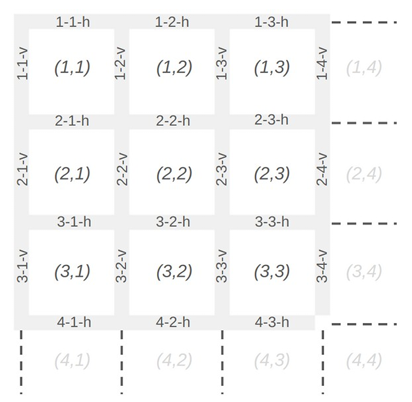
\includegraphics[width=0.7\linewidth]{disTablero}
				\caption{Notar que las líneas punteadas existen en el tablero, pero no pueden ser marcables por los jugadores por estar fuera del rango jugable. Se verifica al realizar la jugada que sea en un lugar válido el movimiento.}
			\end{figure}
			
			\newpage
		\subsection{Fin del juego}
		En este predicado se retorna el final del juego, cuál jugador ganó y con cuantos puntos terminó cada uno. En caso de que no sea el final del juego, el predicado falla.
		
			\subsubsection{Diseño de "Fin del juego"}
			Para el fin del juego se tomó que todas las líneas deben estar marcadas, es decir, una vez que se inicia una partida se debe terminar por completo. Para ello se utiliza un predicado auxiliar que justamente se encarga de verificar que estén todas las líneas marcadas.\\
			
			\subsubsection{Predicado auxiliar 1 - todas\_lineas\_marcadas}
			El predicado auxiliar \textit{todas\_lineas\_marcadas} se encarga de verificar que todas las celdas internas (las que estan entre $1$ y $(N-1)$) estén en marcadas como $c(1,1,\_)$, mientras que las de la última fila $c(1,0,0)$ y las de la última columna $c(0,1,0)$. Es importante que las celdas de los bordes derecho e inferior no tengan un jugador que las haya conquistado, de otra manera no estaría funcionando bien el juego.\\
			
			\subsubsection{Predicado auxiliar 2 - contar\_puntos}
			El otro predicado auxiliar que usa esta función es el de \textit{contar\_puntos} que pasa celda por celda sumando en el contador del jugador correspondiente si está conquistada por él. Por ejemplo, si se tiene la celda $c(\_,\_,1)$, se suma un punto al jugador $1$. Para que esto funcione se debe verificar antes que el juego está terminado de forma que todas las aristas estén marcadas debido a que $c(1,0,1)$ no es una instancia válida de una casilla, así como tampoco lo es $c(0,1,1)$ ni $c(0,0,1)$ (en todas se usa como ejemplo el jugador $1$, pero si en lugar de $1$ fuera $2$ tampoco serían viables estas instancias).
			
		\subsection{Jugada humano}
		En este predicado se realiza una jugada hecha por un humano al ingresar una fila, columna y dirección que corresponden a la arista de la celda que se desea marcar. La dirección indica cual de las 2 aristas marcar en la celda ($h$ para la superior, $v$ para la izquierda). Finalmente se devuelve el tablero actualizado con el movimiento y una lista de las celdas capturadas en caso de ocurrir una captura (notar que como máximo solo se podrán capturar 2 celdas en una misma jugada).
		
			\subsubsection{Diseño de "Jugada humano"}
			Para la función se realizan las siguientes actividades:
			\begin{enumerate}
				\item Validar la jugada: donde se verifica que la arista seleccionada entra dentro de la zona de juego y que dicha arista no esté ya marcada.
				\item Marcar línea: si el movimiento es válido se marca la línea seleccionada.
				\item Verificar las capturas: se determinan las celdas que fueron capturadas si correspondiera, puede no haber capturas, una sola o, como máximo, dos celdas capturadas.
				\item Determinar siguiente turno: de acuerdo a si se realizó alguna captura o no se determina a qué jugador le toca jugar después. Si se realizó por lo menos una captura, el jugador que acaba de marcar línea sigue jugando.
			\end{enumerate}
			
			\subsubsection{Predicado auxiliar 1 - jugada\_valida}
			En este predicado se verifica que, en caso de que la dirección sea $h$, la celda seleccionada caiga entre $(1,1)$ y $(N, N-1)$ (ya que la línea horizontal de la última columna nunca se marca ya que no hay vértices) y el primer item $c(H,\_,\_)$ sea 0, en otro caso falla porque quiere decir que, o bien la celda no entra dentro del rango mencionado, o bien la línea ya fue marcada. En caso de que la dirección sea $v$, el rango de celdas va desde $(1,1)$ y $(N-1,N)$ (última fila no se pueden marcar las líneas verticales) y el segundo item $c(\_,V,\_)$ sea 0.
			
			\subsubsection{Predicado auxiliar 2 - marcar\_linea}
			En este predicado simplemente se marca la línea vertical u horizontal según sea el caso y se reemplaza la celda modificada en el tablero nuevo, previamente ya se verificó que la línea seleccionada está disponible.
			
			\subsubsection{Predicado auxiliar 3 - verificar\_capturas}
			Para este predicado se deben verificar las celdas afectadas por la línea elegida. Las celdas afectadas pueden ser, si la dirección fue $h$, la celda donde se modificó $(F,C)$ y la celda de arriba $(F-1,C)$. En este caso se deben verificar un total de 5 celdas, las dos posible afectadas (posible porque puede ser una celda de la primera fila, en ese caso solo hay una celda afectada), una celda a la derecha por cada celda afectada (para verificar si la línea vertical está marcada o no) y, por último, si la celda inferior a la celda que fue modificada tiene la línea horizontal marcada. En el caso de que la dirección fuese $v$, el pensamiento es análogo, la celda modificada está en $(F,C)$ y la otra posible afectada está en $(F, C-1)$, y se tienen las 2 celdas inferiores a cada una afectada por la línea marcada, además de la que está a la derecha de la modificada.
			
			Para verificar que una celda está capturada se debe dar lo siguiente: para los dos primeros campos de la celda elegida $c(H,V,\_)$ tiene que cumplirse $H=V=1$, que la celda de la derecha tenga $c(\_,1,\_)$ y la celda inferior tenga $c(1,\_,\_)$. Si se cumple todo esto, la celda está capturada, por lo que el tercer campo de la celda $c(\_,\_,J)$ J toma el valor del jugador que realizó el movimiento.
			
			\subsubsection{Predicado auxiliar 4 - determinar\_siguiente\_turno}
			Este predicado simplemente verifica que la lista de celdas capturada esté vacío o no para saber a quien corresponde el siguiente turno, si está vacío al otro jugador, si tiene al menos una captura sigue jugando el mismo jugador que acaba de marcar la línea.
			
		\subsection{Jugada máquina}
		
		
	
\end{document}